% Rapport : historique d'entrainement du modele iter436
% Compilation : pdflatex rapport.tex (deux passes pour la table des matieres)
\documentclass[11pt,a4paper]{article}

\usepackage[utf8]{inputenc}
\usepackage[T1]{fontenc}
\usepackage[french]{babel}
\usepackage{newpxtext}
\usepackage{newpxmath}
\usepackage{microtype}
\usepackage[a4paper,top=2.6cm,bottom=2.8cm,left=2.7cm,right=2.7cm]{geometry}

\usepackage{booktabs}
\usepackage{longtable}
\usepackage{tabularx}
\usepackage{array}
\usepackage{graphicx}
\usepackage{caption}
\usepackage{subcaption}
\usepackage{titlesec}
\usepackage{titletoc}
\usepackage{fancyhdr}
\usepackage{xcolor}
\usepackage[most]{tcolorbox}
\usepackage{tikz}
\usetikzlibrary{arrows.meta,positioning,shapes.geometric,fit,
  backgrounds,calc,patterns}
\usepackage{enumitem}
\usepackage{amsmath}
\usepackage{seqsplit}
\usepackage[hidelinks]{hyperref}

\setlength{\emergencystretch}{2em}

% ---------------------------------------------------------------------------
% Palette et style
% ---------------------------------------------------------------------------
\definecolor{bleu}{HTML}{0B3C5D}
\definecolor{bleuclair}{HTML}{E8F0F5}
\definecolor{gris}{HTML}{444444}
\definecolor{grisfond}{HTML}{F4F4F4}
\definecolor{vert}{HTML}{2E7D32}
\definecolor{rouge}{HTML}{B3261E}
\definecolor{ambre}{HTML}{8A5A00}
\definecolor{ambrefond}{HTML}{FFF6E0}

\captionsetup{font=small,labelfont={bf,color=bleu}}
\addto\captionsfrench{\renewcommand{\figurename}{Figure}}
\addto\captionsfrench{\renewcommand{\tablename}{Tableau}}

\titleformat{\section}
  {\normalfont\Large\bfseries\color{bleu}}{\thesection}{0.8em}{}
\titleformat{\subsection}
  {\normalfont\large\bfseries\color{bleu}}{\thesubsection}{0.7em}{}
\titleformat{\subsubsection}
  {\normalfont\normalsize\bfseries\color{gris}}{\thesubsubsection}{0.6em}{}
\titlespacing*{\section}{0pt}{1.6em}{0.8em}
\titlespacing*{\subsection}{0pt}{1.2em}{0.5em}

\pagestyle{fancy}
\fancyhf{}
\fancyhead[L]{\small\color{gris}\leftmark}
\fancyhead[R]{\small\color{gris}\thepage}
\renewcommand{\headrulewidth}{0.3pt}
\renewcommand{\headrule}{\hbox to\headwidth{\color{bleu!40}\leaders\hrule height \headrulewidth\hfill}}
\setlength{\headheight}{24pt}

% ---------------------------------------------------------------------------
% Encadres
% ---------------------------------------------------------------------------
\newtcolorbox{resume}[1][En résumé]{
  enhanced, breakable, colback=bleuclair, colframe=bleu,
  boxrule=0.8pt, arc=2pt, left=8pt, right=8pt, top=6pt, bottom=6pt,
  fonttitle=\bfseries\small, title={#1},
  attach boxed title to top left={yshift=-2mm, xshift=4mm},
  boxed title style={colback=bleu, arc=1pt, boxrule=0pt},
  before skip=10pt, after skip=10pt}

\newtcolorbox{chiffres}[1][Chiffres clés]{
  enhanced, breakable, colback=white, colframe=bleu,
  boxrule=1pt, arc=2pt, left=10pt, right=10pt, top=8pt, bottom=8pt,
  fonttitle=\bfseries\small, title={#1},
  attach boxed title to top left={yshift=-2mm, xshift=4mm},
  boxed title style={colback=bleu, arc=1pt, boxrule=0pt},
  before skip=10pt, after skip=10pt}

\newtcolorbox{attention}[1][À retenir]{
  enhanced, breakable, colback=ambrefond, colframe=ambre,
  boxrule=0.8pt, arc=2pt, left=8pt, right=8pt, top=6pt, bottom=6pt,
  fonttitle=\bfseries\small, title={#1},
  attach boxed title to top left={yshift=-2mm, xshift=4mm},
  boxed title style={colback=ambre, arc=1pt, boxrule=0pt},
  before skip=10pt, after skip=10pt}

\newcommand{\code}[1]{\texttt{\small #1}}
\newcommand{\chemin}[1]{\texttt{\small\seqsplit{#1}}}
\newcommand{\ok}{\textcolor{vert}{\textbf{OK}}}

% ---------------------------------------------------------------------------
% Metadonnees du document
% ---------------------------------------------------------------------------
\newcommand{\docTitre}{Entraînement du modèle iter436}
\newcommand{\docSousTitre}{1,6 million de parties, 225 millions de positions,
436 itérations de self-play}
\newcommand{\docAuteur}{Mathieu Leclercq}
\newcommand{\docDate}{20 septembre 2026}
\newcommand{\docVersion}{Version 1.0}

\hypersetup{
  pdftitle={\docTitre},
  pdfauthor={\docAuteur},
  pdfsubject={Historique d'entraînement, moteur d'échecs AlphaZero},
  pdfkeywords={AlphaZero, self-play, MCTS, Lichess, ONNX, entraînement}
}

\begin{document}

% ---------------------------------------------------------------------------
% Page de titre
% ---------------------------------------------------------------------------
\begin{titlepage}
\centering
\vspace*{1.5cm}
{\color{bleu}\rule{\textwidth}{1.2pt}}
\vspace{0.8cm}

{\Huge\bfseries\color{bleu} \docTitre\par}
\vspace{0.5cm}
{\Large\color{gris} \docSousTitre\par}

\vspace{0.6cm}
{\large Historique d'entraînement\par}

\vspace{0.4cm}
{\color{bleu}\rule{\textwidth}{0.6pt}}
\vspace{1.2cm}

{\large \docAuteur\par}
{\large \docDate\par}
\vspace{0.3cm}
{\small \docVersion\par}

\vfill

\begin{tcolorbox}[enhanced, colback=grisfond, colframe=gris!50,
  boxrule=0.5pt, arc=2pt, width=0.88\textwidth]
\small
Ce document reconstitue l'entraînement du modèle
\code{2026\_04\_30\_09h53\_iter436\_unsupervised}, celui que le bot utilise
sur Lichess. Il raconte la lignée complète : la première génération de mars,
abandonnée ; le changement d'architecture du 6 avril et la reprise de zéro ;
puis les trois phases qui ont produit le modèle actuel, prétraining Lichess,
affinage sur parties de grands maîtres, et self-play. Tous les chiffres
proviennent des métadonnées des checkpoints, des scripts du dépôt et des
68 runs du projet wandb \code{leclercqmathieu14/alphazero-chess}.
\end{tcolorbox}
\vspace{1cm}
\end{titlepage}

% ---------------------------------------------------------------------------
\tableofcontents
\newpage

\section{Résumé}

Le modèle \code{2026\_04\_30\_09h53\_iter436\_unsupervised} est la deuxième
génération du réseau de LapZero-Chess. Il a été entraîné du 6 au 30 avril 2026
en trois temps : un prétraining supervisé sur des parties Lichess, un court
affinage sur des parties de grands maîtres, puis 436 itérations de self-play.
C'est ce modèle que \code{uci.py} charge aujourd'hui pour jouer sur Lichess
(compte \code{Mboobot}, environ 2\,290 en rapide au moment de la rédaction).

La lignée complète compte en réalité deux générations. La première, entraînée
en mars, a été abandonnée le 6 avril après un changement d'architecture. Une
piste de transfert de poids a été testée ce soir-là, puis écartée : la lignée
retenue est repartie de poids aléatoires, comme le montre la section~2.3.

\begin{chiffres}
\begin{itemize}[leftmargin=1.1em,itemsep=1pt,topsep=2pt]
  \item \textbf{Architecture} : ResNet 10 blocs, 128 filtres, blocs
        Squeeze-and-Excitation, entrée $119 \times 8 \times 8$, policy 4\,672 coups.
  \item \textbf{Parties utilisées} : environ 1,2 million de parties Lichess,
        environ 210\,000 parties de grands maîtres et 211\,000 parties de
        self-play, soit près de 1,6 million.
  \item \textbf{Positions} : 39,9 M uniques pour Lichess, 19,5 M pour les
        grands maîtres, 5,93 M générées par le self-play.
  \item \textbf{Échantillons vus à l'entraînement} (positions présentées au
        réseau, soit lots $\times$ steps) : 79,8 M (Lichess) +
        38,9 M (grands maîtres) + 105,9 M (self-play), soit 224,6 M.
  \item \textbf{Self-play} : 436 itérations, 26\,356 steps d'optimiseur,
        21,7 M coups joués, 5,93 M positions conservées.
  \item \textbf{Niveau estimé} : environ 2\,665 Elo, avec un pic à 2\,892,
        face à Stockfish 2\,600 limité à 200\,000 nœuds.
  \item \textbf{Durée} : du 6 avril 18 h 49 au 30 avril 09 h 53 (heure
        locale), soit environ 23 jours.
\end{itemize}
\end{chiffres}

\section{Chronologie}

\subsection{Deux générations de réseau}

La première génération a été entraînée du 7 au 11 mars : un supervisé sur les
seules parties de grands maîtres (4\,749 steps, une époque), puis un second
passage en ajoutant le jeu de données Lichess (9\,755 steps au total), et un
correctif de la tête de policy (15\,752 steps). Elle a ensuite fait 431
itérations de self-play du 10 mars au 4 avril, atteignant 25\,429 steps
d'optimiseur. Ses checkpoints sont conservés dans \chemin{python\_src/checkpoints}.

Le 6 avril, l'architecture change : des blocs Squeeze-and-Excitation sont
insérés dans chaque bloc résiduel et les têtes sont élargies (commit
\code{75977ce}). Une procédure de transfert de poids est écrite
(\chemin{transfer\_weights.py}) et copie 153 des 187 tenseurs de l'ancien
modèle dans la nouvelle architecture. Deux lancements courts du prétraining
Lichess utilisent ces poids transférés, mais leur perte value reste bloquée
autour de 1,9. La lignée retenue est un troisième lancement, reparti de poids
aléatoires, qui produit le checkpoint conservé
\code{2026\_04\_06\_22h25\_SUPERVISED\_LICHESS\_NEW\_MODEL.ckpt}.

\begin{figure}[h]
\centering
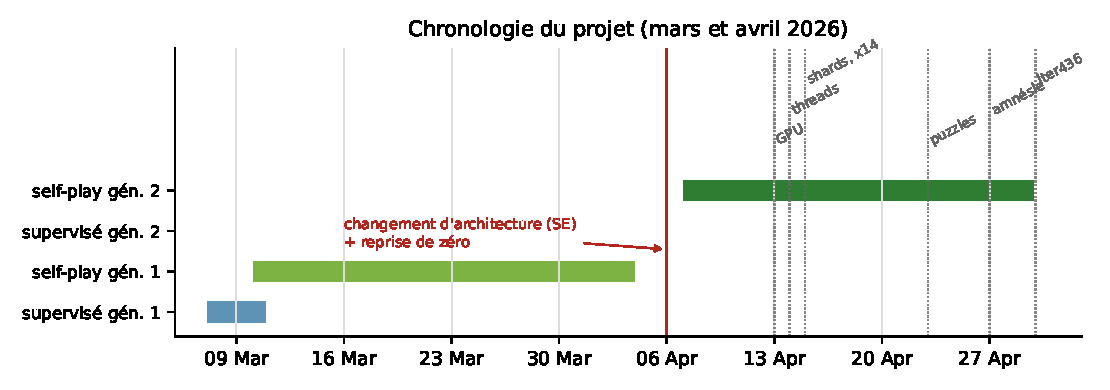
\includegraphics[width=\textwidth]{figures/fig_chronologie.pdf}
\caption{Chronologie du projet en mars et avril 2026. Les événements du
self-play de la génération 2 sont indiqués : self-play batché sur GPU
(13 avril), MCTS multithread (14 avril), buffer en shards et ratio
d'échantillonnage $\times 14$ (15 avril), puzzles tactiques injectés
(23 avril), history dropout (27 avril), dernier checkpoint iter436
(30 avril).}
\label{fig:chronologie}
\end{figure}

\subsection{Les trois phases de la génération retenue}

\begin{table}[h]
\centering
\small
\caption{Phases d'entraînement de la génération retenue. Les positions vues
comptent les époques multiples.}
\label{tab:phases}
\begin{tabularx}{\textwidth}{l >{\raggedright\arraybackslash}p{3.5cm}
    >{\raggedright\arraybackslash}X r r}
\toprule
Phase & Dates (locale) & Données & Positions vues & Steps \\
\midrule
Prétraining Lichess
  & 6 avril, 18 h 49 à 22 h 25
  & 1,2 M de parties, 39,9 M de positions
  & 79,8 M & 19\,495 \\
Affinage grands maîtres
  & 6 avril 22 h 32 à 7 avril 00 h 05
  & 210\,000 parties, 19,5 M de positions
  & 38,9 M & 18\,996 \\
Self-play
  & 7 avril 00 h 34 à 30 avril 09 h 53
  & 211\,000 parties, 5,93 M de positions
  & 105,9 M & 26\,356 \\
\bottomrule
\end{tabularx}
\end{table}

Le prétraining Lichess a en réalité demandé trois lancements successifs
(18 h 49, 19 h 16 et 19 h 33) ; seul le troisième, long de 2 h 52, a produit le
checkpoint conservé. L'affinage sur les grands maîtres a duré 1 h 33. Le
self-play a occupé les 23 jours suivants, en 26 lancements qui reprenaient
chacun le dernier checkpoint du précédent. Le détail de ces 26 lancements est
donné en annexe~A.

\section{Supervisé : Lichess puis grands maîtres}

\subsection{Prétraining Lichess}

Le jeu de données vient du dump Lichess \code{standard rated} de février 2026,
filtré sur les deux joueurs à 1\,800 Elo ou plus
(\chemin{extract\_pgn\_from\_lichess.py}). Le fichier conservé,
\chemin{top\_games\_quality.pgn}, pèse 2,37 Go et contient exactement
1\,000\,000 de parties. Il a été converti en shards binaires
(\chemin{convert\_pgn\_to\_binary.py}) : des fichiers \code{.npz} de 500
parties, environ 16\,600 positions chacun, avec le tenseur
$119 \times 8 \times 8$ en \code{uint8}, l'indice de policy et le résultat.

Le dernier shard conservé porte l'indice 2399, ce qui indique environ
2\,400 shards, soit environ 1,2 million de parties et 39,9 M de positions.
Le fichier PGN conservé (1 M de parties) est donc légèrement plus petit que
l'entrée de conversion ; ce point est discuté en section~5.

L'entraînement utilise des shards mélangés (\chemin{sharded\_dataset.py}),
un lot de 4\,096, Adam à $10^{-3}$ et la précision mixte 16 bits. Le run
retenu a tourné 2 h 52 et s'est arrêté au bout de deux époques complètes,
19\,495 steps, soit 79,8 M d'échantillons vus.

\begin{figure}[h]
\centering
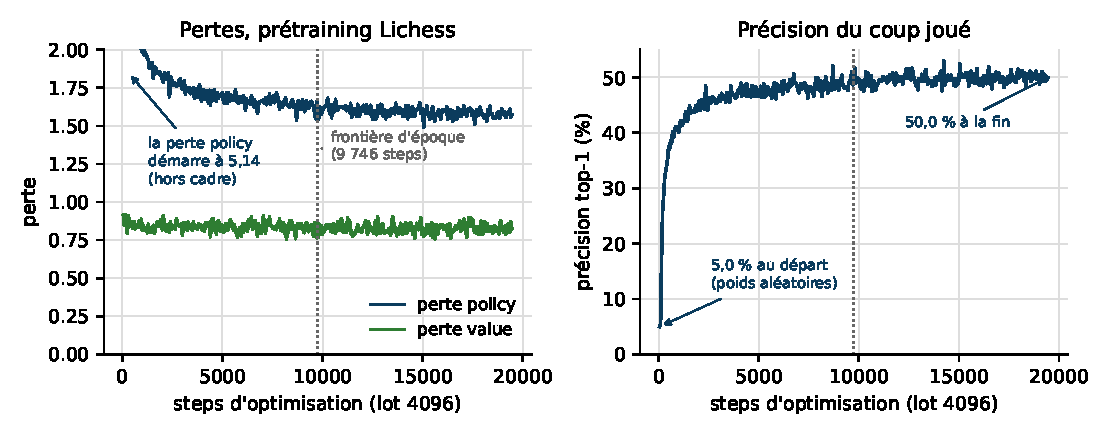
\includegraphics[width=\textwidth]{figures/fig_supervise_lichess.pdf}
\caption{Prétraining Lichess, run \code{jhqhhx5q}. À gauche, les pertes
policy et value sur une échelle linéaire plafonnée à 2, pour comparer
directement avec la figure~\ref{fig:gm} ; la perte policy démarre à 5,14,
au-dessus du cadre. La ligne pointillée marque la frontière d'époque à
9\,746 steps. À droite, la précision top-1 du coup joué, de 5,0 \% au départ
(poids aléatoires) à 50,0 \% à la fin.}
\label{fig:lichess}
\end{figure}

Les courbes de la figure~\ref{fig:lichess} sont le meilleur certificat de la
reprise de zéro : la précision démarre à 5 \%, la valeur typique d'un réseau
non entraîné, et non à 30 ou 40 \% comme pour un modèle déjà joueur. La perte
policy chute de 5,14 à 1,57, la perte value de 0,91 à 0,82. La petite marche
visible sur la perte policy au voisinage de la ligne pointillée correspond au
changement d'époque ; elle est bénigne et vient du brassage des shards.

\subsection{Affinage sur les parties de grands maîtres}

La deuxième phase reprend le checkpoint Lichess et l'affine sur les parties de
grands maîtres téléchargées depuis pgnmentor
(\chemin{download\_pgns.py}), nettoyées et dédoublonnées en un fichier par
partie (\chemin{clean\_pgns.7z}). Le script
(\chemin{train\_supervised.py}) change aussi de format : il lit directement
les PGN, sans passer par les shards, avec un lot de 2\,048.

Le jeu conservé dans \chemin{docs/clean\_pgns.7z} ne contient que 56\,562
parties, mais il s'agit d'un instantané partiel de mars. La taille réelle de
l'époque d'affinage se lit dans le checkpoint : 9\,498 lots de 2\,048, soit
19,45 M de positions par époque. Avec une moyenne de 91,5 plies par partie
(mesurée sur l'archive), cela représente environ 210\,000 parties.

Le run a duré 1 h 33 et fait exactement deux époques, 18\,996 steps, soit
38,9 M d'échantillons vus. Il s'arrête à l'époque 3 du compteur Lightning,
qui avait été hérité du checkpoint Lichess.

\begin{figure}[h]
\centering
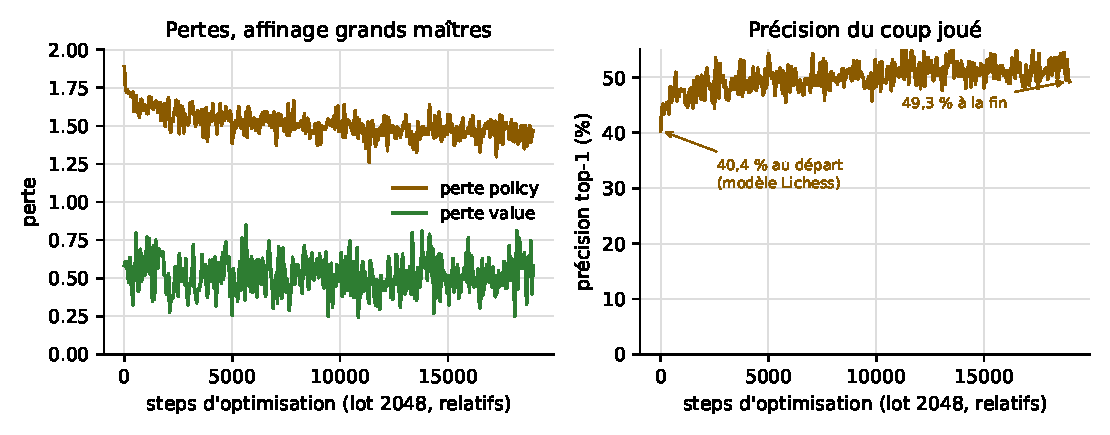
\includegraphics[width=\textwidth]{figures/fig_supervise_gm.pdf}
\caption{Affinage sur les grands maîtres, run \code{ifvh81l0}. Les steps sont
relatifs au début de l'affinage. La précision passe de 40,4 \% (modèle
Lichess) à 49,3 \%. La perte value reste plate autour de 0,58.}
\label{fig:gm}
\end{figure}

La figure~\ref{fig:gm} montre un régime différent du prétraining : à
l'échelle de ces deux époques, la perte policy baisse (1,89 à 1,47) et la
précision progresse de 40,4 \% à 49,3 \%, tandis que la perte value ne bouge
pratiquement pas (0,58). Autrement dit, l'affinage sert surtout à ajuster la
politique sur un style de jeu plus propre et plus tactique, pas à recalibrer
la valeur.

\subsection{Le transfert de poids testé puis abandonné}

Le soir du 6 avril, trois lancements du prétraining Lichess se succèdent. Les
deux premiers utilisent les poids transférés depuis l'ancien modèle ; le
troisième part de zéro. La figure~\ref{fig:transfert} compare les trois.

\begin{figure}[h]
\centering
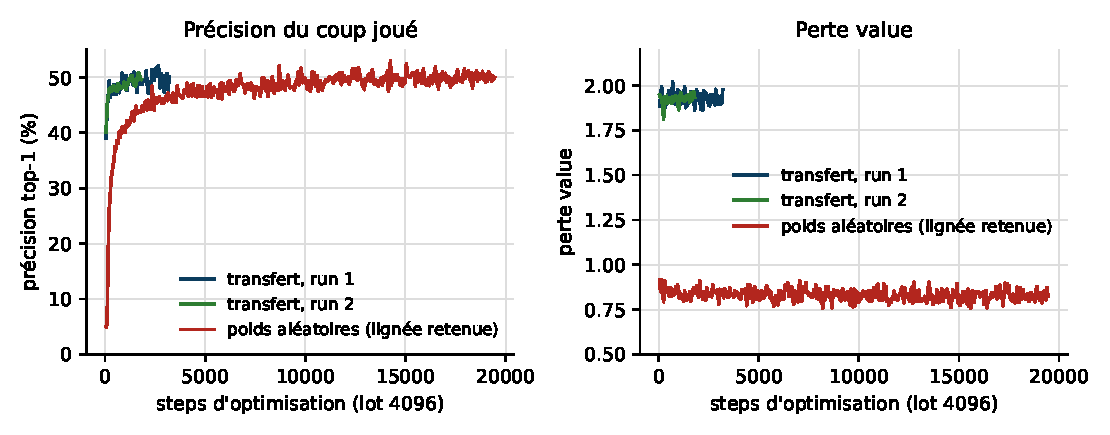
\includegraphics[width=\textwidth]{figures/fig_transfert.pdf}
\caption{Les trois lancements du prétraining Lichess du 6 avril. À gauche, la
précision top-1 : elle démarre à 39 et 40 \% pour les runs avec transfert, à
5 \% pour le run reparti de zéro. À droite, la perte value : elle reste
bloquée autour de 1,9 pour les runs transférés, contre 0,8 pour le run
retenu.}
\label{fig:transfert}
\end{figure}

Les deux runs transférés ont une précision de départ élevée (39 et 40 \%), ce
qui confirme que le transfert fonctionne pour l'essentiel du réseau. Mais leur
perte value reste autour de 1,9 pendant tout le run, deux fois pire qu'un
réseau aléatoire, alors que le run reparti de zéro la fait descendre sous
0,85. La tête de value transférée est donc inadaptée à la nouvelle
architecture, ou à la convention de signe du jeu de données. Les deux runs
ont été interrompus après 3\,200 et 1\,800 steps ; le troisième, sans
transfert, a été mené au bout.

\begin{attention}
La lignée du modèle actuel ne contient pas les poids transférés. Les fichiers
\code{modele\_generation0\_init.pt} et
\code{alphazero-supervised-step=3000.ckpt}, dans le dossier
\chemin{python\_src/checkpoints}, conservent la trace de cet essai, mais ils ne
font pas partie de l'ascendance de l'iter436. Le modèle est bien reparti de
zéro au stade supervisé.
\end{attention}

\section{Self-play}

Le self-play démarre le 7 avril à 00 h 34, à partir du checkpoint de
l'affinage converti au format du self-play
(\chemin{convert\_ckpt.py}, sortie
\chemin{2026\_04\_07\_00h10\_UNSUPERVISED\_NEW\_MODEL.pt}).

\subsection{La recette}

\begin{itemize}[leftmargin=1.2em,itemsep=2pt,topsep=2pt]
  \item \textbf{Parties} : 512 par itération, sauf les itérations 27 à 37
        (256 par itération, pendant la transition vers le self-play batché
        sur GPU).
  \item \textbf{Recherche} : MCTS, 700 simulations sur les coups lents et
        100 sur les coups rapides, avec 25 \% de coups lents. Table de
        transposition de 4 millions d'entrées. Génération des parties en C++
        avec inférence batchée sur GPU à partir du 13 avril.
  \item \textbf{Entraînement} : AdamW ($\text{weight decay} = 10^{-4}$),
        learning rate $5 \cdot 10^{-6}$ au premier run, puis $5 \cdot 10^{-5}$,
        $2 \cdot 10^{-5}$ et $4 \cdot 10^{-5}$ à partir du 14 avril. Lot de
        2\,048 puis 4\,096, précision mixte 16 bits.
  \item \textbf{Buffer} : 750\,000 positions sur disque, en shards. Chaque
        itération échantillonne 14 fois le volume de positions qu'elle vient
        de générer.
  \item \textbf{Évaluation} : 16 parties contre Stockfish limité à
        200\,000 nœuds toutes les 8 itérations, avec une ancre montée de
        2\,200 à 2\,300, 2\,450 puis 2\,600 Elo.
\end{itemize}

\subsection{Déroulé et volumes}

Les 436 itérations se répartissent sur 26 lancements, chacun reprenant le
checkpoint du précédent (annexe~A). Au total : 211\,200 parties générées,
5,93 M de positions conservées pour l'entraînement, 21,7 M de coups joués et
26\,356 steps d'optimiseur, soit 105,9 M d'échantillons vus.

\begin{figure}[h]
\centering
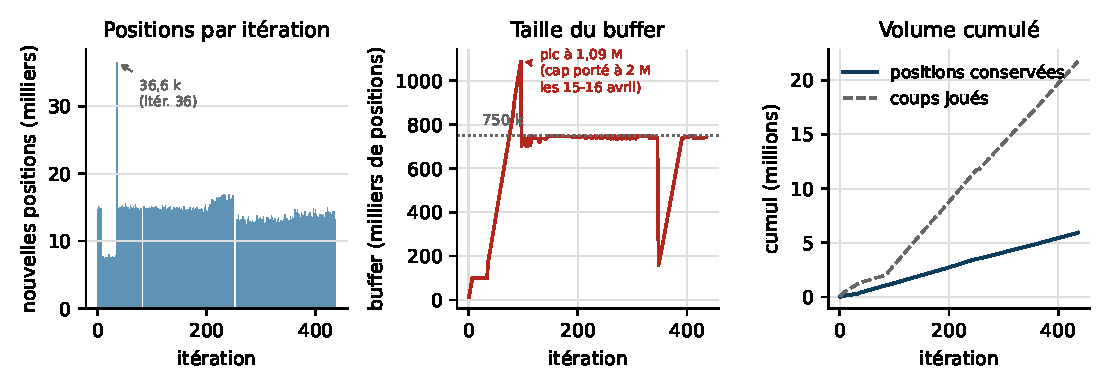
\includegraphics[width=\textwidth]{figures/fig_selfplay_volume.pdf}
\caption{Volume du self-play. À gauche, les positions générées par itération
(le pic de l'itération 36 vient d'un lancement qui en a conservé davantage).
Au centre, la taille du buffer, avec un pic à 1,09 M quand le plafond a été
porté temporairement à 2 M les 15 et 16 avril. À droite, les cumuls : les
positions conservées (coups lents) et l'ensemble des coups joués.}
\label{fig:volume-selfplay}
\end{figure}

Le rapport entre les deux courbes du panneau de droite est cohérent avec la
recette : seuls les coups joués sous recherche lente sont conservés comme
positions d'entraînement, soit environ un quart des coups. Le buffer, lui,
reste plein à 750\,000 positions : le modèle ne réapprend donc jamais deux
fois le même échantillon, il tourne sur ses parties les plus récentes.

\subsection{Pertes et learning rate}

\begin{figure}[h]
\centering
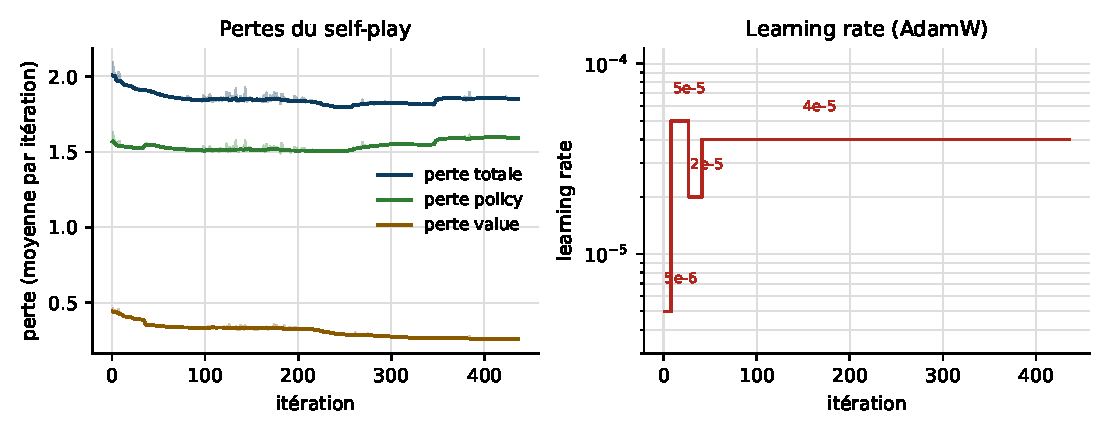
\includegraphics[width=\textwidth]{figures/fig_selfplay_pertes.pdf}
\caption{À gauche, les pertes du self-play, valeurs brutes (traits fins) et
médiane glissante sur 21 itérations (traits épais). À droite, l'évolution du
learning rate.}
\label{fig:pertes-selfplay}
\end{figure}

La perte totale passe d'environ 1,94 à 1,86 en médiane. La perte value, elle,
baisse nettement, d'environ 0,41 à 0,26 : le modèle devient sensiblement
meilleur pour prédire le résultat des positions. La perte policy reste
autour de 1,54 à 1,60, avec une légère remontée.

\begin{attention}
La perte policy du self-play n'est pas comparable d'une itération à l'autre :
la cible est la politique de recherche du modèle lui-même et le jeu de
données glisse en permanence. Une remontée de cette courbe ne signifie pas
une régression, c'est aussi le signe que les positions deviennent plus
difficiles. La perte value, ancrée sur le résultat réel des parties, est le
meilleur indicateur de progression de cette phase.
\end{attention}

\subsection{Qualité des parties}

\begin{figure}[h]
\centering
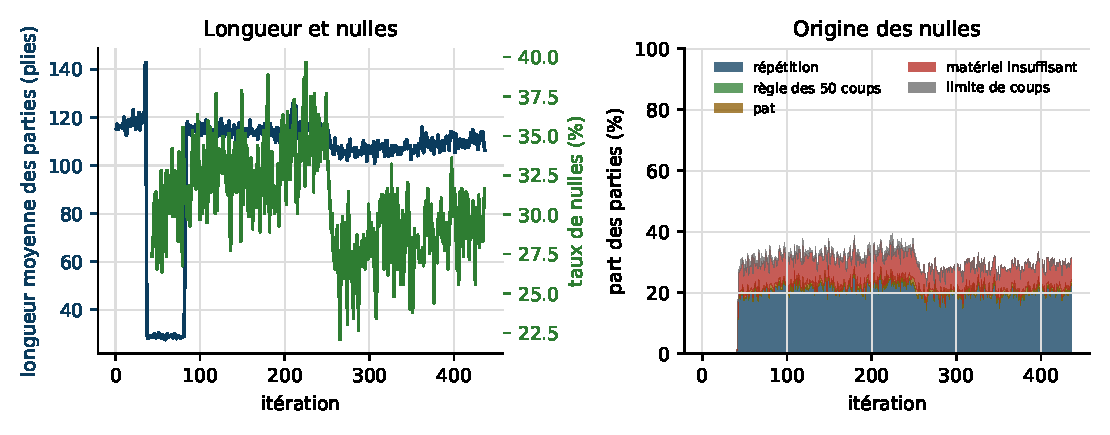
\includegraphics[width=\textwidth]{figures/fig_selfplay_qualite.pdf}
\caption{À gauche, la longueur moyenne des parties (en plies) et le taux de
nulles. À droite, la décomposition des nulles par cause.}
\label{fig:qualite-selfplay}
\end{figure}

Les parties durent environ 117 plies au début, puis se stabilisent autour de
105 à 110 plies. Le taux de nulles reste autour de 30 \%, dominé par les
répétitions (environ 20 \% des parties) et le matériel insuffisant (environ
8 \%). La règle des 50 coups, le pat et la limite de coups restent marginaux.
Les pics de nulles par répétition autour des itérations 60 à 100
correspondent aux périodes où le tirage de Dirichlet et la température
favorisaient l'exploration.

\subsection{Niveau face à Stockfish}

\begin{figure}[h]
\centering
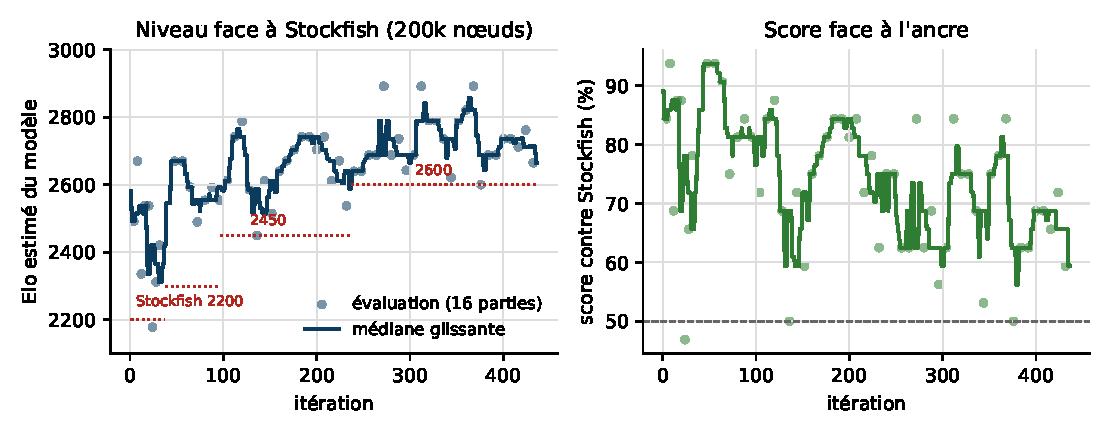
\includegraphics[width=\textwidth]{figures/fig_elo.pdf}
\caption{Niveau estimé face à Stockfish, 200\,000 nœuds et 16 parties par
évaluation. La ligne pointillée rouge indique l'Elo de l'ancre, qui change
en cours de route : les estimations ne sont donc pas sur la même échelle
d'une période à l'autre. À droite, le score brut contre l'ancre.}
\label{fig:elo}
\end{figure}

La première évaluation, à l'itération 4, donne 2\,492 Elo. La dernière, à
l'itération 432, donne 2\,665 Elo ; le maximum observé est 2\,892. La série
est très bruitée : chaque point ne repose que sur 16 parties, ce qui donne
une incertitude de l'ordre de $\pm 150$ Elo. Les paliers visibles dans le
score (60, 75, 85 \%) suivent surtout les changements d'ancre, et non des
sauts de niveau du modèle. La tendance de fond reste une progression claire
entre le début du self-play (autour de 2\,490) et la fin (autour de 2\,650),
avec des passages réguliers au-dessus de 2\,750.

\section{Bilan des volumes}

\begin{figure}[h]
\centering
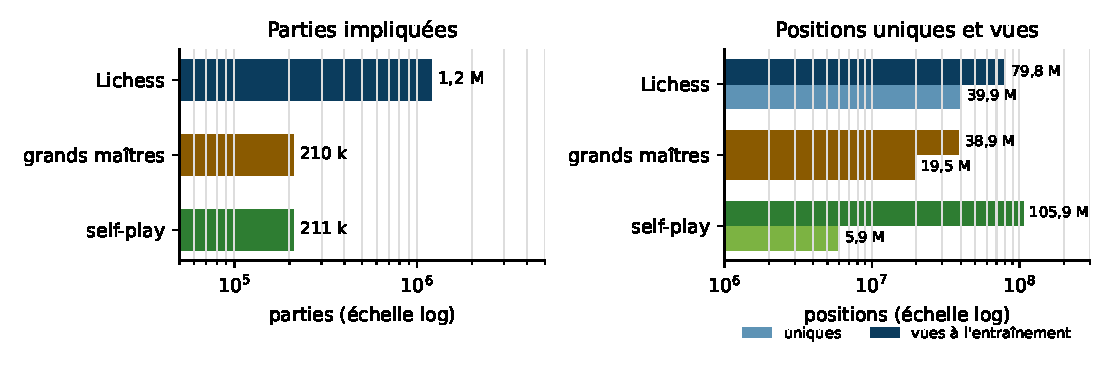
\includegraphics[width=\textwidth]{figures/fig_volumes.pdf}
\caption{À gauche, le nombre de parties par phase. À droite, les positions
uniques et le nombre de positions effectivement vues à l'entraînement
(échelle logarithmique). Pour le self-play, les positions « uniques » sont
les positions conservées, soit les coups joués sous recherche lente.}
\label{fig:volumes}
\end{figure}

\begin{table}[h]
\centering
\small
\caption{Récapitulatif des trois phases de la génération retenue.}
\label{tab:volumes}
\begin{tabular}{l r r r r}
\toprule
Phase & Parties & Positions uniques & Époques & Échantillons vus \\
\midrule
Lichess          & 1\,200\,000 & 39,9 M & 2  & 79,8 M \\
Grands maîtres   & 210\,000    & 19,5 M & 2  & 38,9 M \\
Self-play        & 211\,200    & 5,93 M & 18 & 105,9 M \\
\bottomrule
\end{tabular}
\end{table}

Le tableau~\ref{tab:volumes} et la figure~\ref{fig:volumes} racontent la même
histoire en deux temps. Les deux phases supervisées apportent l'essentiel de
la \emph{diversité} : 1,4 million de parties humaines, dont 39,9 M de positions
Lichess et 19,5 M de positions de grands maîtres, chacune parcourue deux fois.

\begin{chiffres}[Comment lire ces chiffres]
Une \emph{position unique} est une position stockée une fois dans un jeu de
données. Un \emph{échantillon vu} est une position présentée au réseau lors
d'un pas d'optimisation, c'est-à-dire une mise à jour des poids :
\[
\text{échantillons vus} = \text{steps} \times \text{taille de lot}.
\]
Un lot contient ici 2\,048 ou 4\,096 échantillons ; un échantillon n'est donc
pas un lot. Le nombre d'échantillons vus dépasse le nombre de positions
uniques dès que le même jeu de données est parcouru plusieurs fois, que ce
soit par époques multiples ou par rééchantillonnage du buffer. La vérification
est directe : $19\,495 \times 4\,096 = 79,8$ M pour Lichess et
$18\,996 \times 2\,048 = 38,9$ M pour les grands maîtres, soit deux époques
dans les deux cas.
\end{chiffres}

Le self-play, lui, n'apporte que 5,93 M de positions nouvelles, mais chaque
position est revue en moyenne 18 fois au fil des itérations. C'est la phase la
plus coûteuse en calcul pour le moins de données brutes, ce qui est le
principe même d'AlphaZero : la donnée est produite puis digérée en continu par
le modèle.

En cumulé, le modèle a vu 224,6 M de positions pendant son entraînement, dont
47 \% proviennent du self-play et 53 \% du supervisé. Le rapport entre les deux
mondes est un équilibre classique : assez de supervisé pour apprendre les
fondamentaux, assez de self-play pour dépasser la qualité des parties
humaines utilisées.

\begin{resume}
À retenir en trois points :
\begin{itemize}[leftmargin=1.1em,itemsep=1pt,topsep=2pt]
  \item le modèle est reparti de zéro le 6 avril, après avoir changé
        d'architecture (blocs SE) ; le transfert de poids testé ce soir-là a
        été abandonné à cause d'une tête de value inadaptée ;
  \item le supervisé apporte 1,4 M de parties humaines et 59,4 M de positions
        uniques ; le self-play ajoute 211\,000 parties et 5,93 M de positions,
        revues 18 fois en moyenne ;
  \item en 23 jours, le niveau estimé passe d'environ 2\,490 à environ
        2\,650 Elo, avec un pic à 2\,892 face à Stockfish 2\,600.
\end{itemize}
\end{resume}

\section{Limites et zones d'ombre}

\begin{itemize}[leftmargin=1.2em,itemsep=3pt,topsep=2pt]
  \item \textbf{Taille exacte du jeu Lichess.} Le fichier PGN conservé
        contient 1\,000\,000 de parties, mais la longueur d'époque lue dans le
        checkpoint implique environ 2\,400 shards, soit environ 1,2 M de
        parties. L'entrée de conversion était donc légèrement plus grande que
        le fichier conservé, ou celui-ci a été ré-extrait plus tard avec un
        plafond à 1 M.

  \item \textbf{Parties de grands maîtres.} L'archive
        \chemin{docs/clean\_pgns.7z} ne contient que 56\,562 parties, un
        instantané de mars. Le nombre d'environ 210\,000 parties est estimé à
        partir des 19,45 M de positions par époque et de la longueur moyenne
        mesurée sur l'archive (91,5 plies).

  \item \textbf{Checkpoints intermédiaires manquants.} Plusieurs checkpoints
        intermédiaires cités par les runs (iter180, iter346, iter347, etc.) ne
        sont plus présents dans \chemin{python\_src/checkpoints}. Seuls les
        jalons conservés par l'auteur sont disponibles.

  \item \textbf{Itérations sans journal.} Neuf itérations n'ont pas de
        données wandb (42, 82, 83, 179, 251 à 254 et 347), en général après un
        run interrompu. La chaîne des runs a été reconstituée par le champ
        \code{checkpoint\_path} de chaque configuration ; les volumes cumulés
        sont donc des minorants stricts.

  \item \textbf{Elo estimé, pas Elo mesuré.} Les évaluations font 16 parties
        contre un Stockfish limité en nœuds (200\,000). Le bruit est de
        l'ordre de $\pm 150$ Elo par point, et l'ancre change quatre fois en
        cours de route, ce qui décale l'échelle. Le chiffre de 2\,665 Elo est
        une estimation face à cette ancre, pas un classement de tournoi.

  \item \textbf{Pertes non comparables entre phases.} La perte policy du
        self-play dépend de la politique de recherche du modèle, qui évolue
        avec lui ; elle ne se compare ni à celle du supervisé, ni d'une
        itération à l'autre. Seules les pertes value du supervisé et les
        taux de victoire sont directement interprétables.

  \item \textbf{Ancienne génération.} Les chiffres de la génération de mars
        sont exacts (lus dans les checkpoints) mais son historique de runs
        n'a pas été audité en détail ici : elle n'a servi qu'à documenter
        l'origine du transfert abandonné.
\end{itemize}


\appendix
\section{Runs du self-play de la génération retenue}

Les 26 lancements de self-play, dans l'ordre chronologique. Les heures sont
locales (UTC+2). Les itérations indiquent la plage réellement journalisée dans
chaque run. Le code est l'identifiant wandb du run.

\begin{longtable}{l r r r l r l}
\caption{Runs de self-play de la génération retenue.}
\label{tab:runs-selfplay} \\
\toprule
Date & Itér. début & Itér. fin & Parties/itér. & LR & Lot & Run \\
\midrule
\endfirsthead
\toprule
Date & Itér. début & Itér. fin & Parties/itér. & LR & Lot & Run \\
\midrule
\endhead
\bottomrule
\endfoot
07 avril 00:34 & 1 & 7 & 512 & 5e-6 & 1024 & \code{m8pz5otu} \\
08 avril 12:43 & 8 & 26 & 256 & 5e-5 & 2048 & \code{vpbjbf7j} \\
09 avril 16:44 & 27 & 30 & 256 & 2e-5 & 2048 & \code{uqrzrwut} \\
12 avril 19:17 & 31 & 34 & 256 & 2e-5 & 2048 & \code{nsgcxhaj} \\
13 avril 17:39 & 35 & 36 & 256 & 2e-5 & 2048 & \code{17lj9pqz} \\
13 avril 22:46 & 37 & 37 & 32 & 2e-5 & 2048 & \code{hus8s590} \\
13 avril 23:12 & 37 & 37 & 512 & 2e-5 & 2048 & \code{m1mi6ixe} \\
14 avril 13:33 & 38 & 40 & 512 & 2e-5 & 2048 & \code{csggla4i} \\
14 avril 17:50 & 41 & 41 & 512 & 4e-5 & 4096 & \code{ys4kv1lb} \\
14 avril 21:05 & 43 & 69 & 512 & 4e-5 & 4096 & \code{ef1nhupv} \\
16 avril 00:37 & 70 & 81 & 512 & 4e-5 & 4096 & \code{x664bpmu} \\
16 avril 13:44 & 84 & 96 & 512 & 4e-5 & 4096 & \code{ecxcsfro} \\
17 avril 00:34 & 97 & 110 & 512 & 4e-5 & 4096 & \code{44q8hjkp} \\
17 avril 13:07 & 111 & 145 & 512 & 4e-5 & 4096 & \code{wy05jkb6} \\
18 avril 20:33 & 146 & 178 & 512 & 4e-5 & 4096 & \code{ousba3tl} \\
20 avril 13:45 & 180 & 180 & 512 & 4e-5 & 4096 & \code{4z3j86bz} \\
20 avril 14:34 & 181 & 208 & 512 & 4e-5 & 4096 & \code{04jv9d6n} \\
21 avril 21:12 & 209 & 213 & 512 & 4e-5 & 4096 & \code{x0h5194i} \\
22 avril 01:31 & 214 & 236 & 512 & 4e-5 & 4096 & \code{s6aa010p} \\
23 avril 00:44 & 237 & 250 & 512 & 4e-5 & 4096 & \code{l4hysg2e} \\
23 avril 17:08 & - & - & 512 & 4e-5 & 4096 & \code{t6t1x00e} \\
23 avril 17:23 & 255 & 261 & 512 & 4e-5 & 4096 & \code{oghdwvmm} \\
23 avril 23:25 & 262 & 316 & 512 & 4e-5 & 4096 & \code{g2el0853} \\
26 avril 18:18 & 317 & 346 & 512 & 4e-5 & 4096 & \code{24gfg9iw} \\
27 avril 21:03 & 348 & 405 & 512 & 4e-5 & 4096 & \code{tsndt3dr} \\
30 avril 09:53 & 406 & 436 & 512 & 4e-5 & 4096 & \code{225nnvy4} \\
\end{longtable}

\section{Runs supervisés et génération précédente}

\begin{table}[h]
\centering
\small
\caption{Les quatre runs supervisés du 6 avril.}
\label{tab:runs-supervise}
\begin{tabular}{l l r r r}
\toprule
Run & Initialisation & Steps & Précision & Perte value \\
\midrule
\code{hamgvtvc} & poids transférés & 3\,199 & 39,0 \% $\to$ 50,1 \% & 1,88 $\to$ 1,98 \\
\code{c3t86nnd} & poids transférés & 1\,799 & 40,1 \% $\to$ 49,7 \% & 1,95 $\to$ 1,94 \\
\code{jhqhhx5q} & aléatoire (retenu) & 19\,495 & 5,0 \% $\to$ 50,0 \% & 0,91 $\to$ 0,82 \\
\code{ifvh81l0} & affinage GM (retenu) & 18\,996 & 40,4 \% $\to$ 49,3 \% & 0,58 $\to$ 0,58 \\
\bottomrule
\end{tabular}
\end{table}

\begin{table}[h]
\centering
\small
\caption{Génération précédente (premier réseau, sans blocs SE), conservée
comme référence.}
\label{tab:gen1}
\begin{tabular}{l l r}
\toprule
Date & Étape & Steps (cumulés) \\
\midrule
7 mars 2026  & supervisé, grands maîtres seuls & 4\,749 \\
9 mars 2026  & ajout du jeu Lichess & 9\,755 \\
11 mars 2026 & correctif de la tête de policy & 15\,752 \\
10 mars au 4 avril 2026 & self-play, 431 itérations & 25\,429 \\
\bottomrule
\end{tabular}
\end{table}

\section{Sources et reproduction}

\subsection{D'où viennent les chiffres}

\begin{itemize}[leftmargin=1.2em,itemsep=3pt,topsep=2pt]
  \item \textbf{Checkpoints supervisés} (Lightning) : les champs
        \code{epoch}, \code{global\_step} et l'état des boucles
        (\code{loops.fit\_loop}) donnent le nombre exact de steps, le nombre
        de lots par époque et les compteurs d'époque. Lecture par
        \code{torch.load} avec \code{weights\_only=False}.
  \item \textbf{Checkpoints self-play} (\code{.pt}) : les clés
        \code{iteration} et \code{global\_step} donnent l'état exact de chaque
        jalon (par exemple \code{iteration=436}, \code{global\_step=26356}).
  \item \textbf{Shards binaires} : les tailles et les tenseurs lus dans
        \chemin{Downloads/dataset\_shards} donnent la taille d'époque du
        prétraining (chaque shard de 500 parties contient environ 16\,600
        positions).
  \item \textbf{Wandb} : le projet
        \href{https://wandb.ai/leclercqmathieu14/alphazero-chess}{%
        leclercqmathieu14/alphazero-chess} contient les 68 runs de mars et
        avril. Un export local complet a été réalisé dans
        \chemin{out/wandb\_export} (configurations, résumés, historiques CSV,
        journaux de sortie).
\end{itemize}

\subsection{Exporter wandb en local}

L'export a été produit par \chemin{out/fetch\_wandb.py} (clé API lue depuis
\chemin{out/wandb\_key.txt}, ce dossier est ignoré par git), puis agrégé par
\chemin{out/aggregate.py} en deux fichiers de travail :
\chemin{merged\_selfplay.csv} (une ligne par itération) et
\chemin{runs\_augmented.json} (une entrée par lancement, avec la plage
d'itérations couverte).

\subsection{Regénérer les figures}

Depuis le dossier \chemin{docs/rapports/2026-04-entrainement-iter436} :

\begin{verbatim}
python figures/generer_figures.py
\end{verbatim}

Le script lit \chemin{out/wandb\_export} et écrit les neuf figures PDF dans
\chemin{figures/}. Il demande \code{matplotlib} et \code{numpy}
(\code{python3} sur la machine de rédaction).

\subsection{Documentation liée}

\begin{itemize}[leftmargin=1.2em,itemsep=2pt,topsep=2pt]
  \item \chemin{docs/training-history.md} : la même reconstitution en
        anglais, au format court.
  \item \chemin{python\_src/train\_supervised.py} et
        \chemin{python\_src/train\_self\_play.py} : les deux scripts
        d'entraînement.
  \item \chemin{python\_src/checkpoints/} : les jalons conservés de la
        génération 1 et de la génération 2.
  \item \chemin{CHANGELOG.md} : les jalons techniques du projet depuis 2022.
\end{itemize}


\end{document}
